% V-1-4 Постер (A3 хэвтээ, dark bento загвар)
% Байгуул: xelatex poster.tex
\documentclass{article}
\usepackage[a3paper,landscape,margin=8mm]{geometry}
\usepackage{fontspec}
\usepackage{graphicx}
\usepackage{tikz}
\usepackage{enumitem}
\usepackage{amssymb}
\usepackage[most]{tcolorbox}
\usepackage{xcolor}
\usetikzlibrary{arrows.meta,positioning,shadings}

\graphicspath{{../report_src/img/}}

% --- Фонт: гарчиг (латин) Avenir Next, монгол Helvetica Neue, код Menlo ---
\setmainfont{Helvetica Neue}
\newfontfamily\disp{Avenir Next}[Scale=MatchLowercase]
\newfontfamily\mono{Menlo}[Scale=MatchLowercase]

% --- Өнгөний палитр (dark) ---
\definecolor{bgdark}{HTML}{0B1220}
\definecolor{card}{HTML}{121C30}
\definecolor{cardline}{HTML}{263850}
\definecolor{cyanA}{HTML}{38BDF8}
\definecolor{amberA}{HTML}{FBBF24}
\definecolor{violetA}{HTML}{A78BFA}
\definecolor{greenA}{HTML}{34D399}
\definecolor{txtw}{HTML}{F1F5F9}
\definecolor{muted}{HTML}{8FA3BF}

\pagecolor{bgdark}
\color{txtw}
\pagestyle{empty}
\setlength{\parindent}{0pt}

% --- Кардын стиль ---
\tcbset{
  poster/.style={
    enhanced jigsaw, colback=card, colframe=cardline,
    boxrule=0.7pt, arc=3.5mm, left=4mm, right=4mm, top=3mm, bottom=3mm,
    fonttitle=\fontsize{11}{13}\selectfont,
    colbacktitle=card, titlerule=0.4mm, toptitle=2.5mm, bottomtitle=1.5mm,
    coltitle=cyanA,
    title={\bfseries #1},
  },
}

% --- Бүтцийн chip ---
\newcommand{\chip}[2]{%
\tcbox[on line, enhanced, colback=bgdark!82!card, colframe=cardline, arc=2mm,
  boxsep=0.8mm, left=1.2mm, right=1.2mm, top=0.5mm, bottom=0.5mm,
  boxrule=0.6pt]{%
  {\fontsize{9.2}{11}\selectfont\textcolor{#1}{$\bullet$}\;{\color{txtw}#2}}}}

% --- Том статистик тоо ---
\newcommand{\stat}[2]{%
\begin{minipage}[t]{41mm}
\centering
{\disp\fontsize{19}{23}\selectfont\bfseries\color{amberA}#1\par}
\vspace{0.5mm}
{\fontsize{8}{10}\selectfont\color{muted}#2\par}
\end{minipage}}

% --- Цагаан дэвсгэрт дээрх screenshot ---
\newcommand{\shot}[2]{%
  \begin{tcolorbox}[enhanced, colback=white, colframe=white, arc=1.8mm,
    left=0.8mm, right=0.8mm, top=0.8mm, bottom=0.8mm, boxsep=0mm]
    \centering #1
  \end{tcolorbox}
  {\centering{\fontsize{7.6}{9.4}\selectfont\color{muted} #2\par}}}

\begin{document}

% --- Зөөлөн гэрэлтэлт (дэвсгэрийн гоёлчи) ---

\begin{tikzpicture}[remember picture, overlay]
  \shade[inner color=cyanA!16, outer color=bgdark, opacity=0.75]
    (current page.north east) circle (130mm);
  \shade[inner color=violetA!14, outer color=bgdark, opacity=0.75]
    ([xshift=25mm]current page.south west) circle (120mm);
\end{tikzpicture}

% ===========================================================================
% HERO
% ===========================================================================
\begin{tcolorbox}[enhanced jigsaw, colback=card, colframe=cardline, boxrule=0.7pt,
  arc=4mm, left=6mm, right=6mm, top=3mm, bottom=3mm, height=46mm, valign=center]
\begin{minipage}[c]{296mm}
{\fontsize{9.5}{12}\selectfont\bfseries\color{cyanA}ШУТИС \;·\; МЭДЭЭЛЭЛ, ХОЛБООНЫ ТЕХНОЛОГИЙН СУРГУУЛЬ \;·\; ҮЙЛДЛИЙН СИСТЕМ F.CSM302 \;·\; БИЕ ДААЛТ 2 \;·\; БАГ V-1-4\par}
\vspace{2.5mm}
{\disp\fontsize{34}{38}\selectfont\bfseries\color{txtw}KERNEL DATA STRUCTURES\par}
\vspace{1.5mm}
{\fontsize{13}{16}\selectfont\color{txtw}\bfseries Linux kernel-ийн 9 өгөгдлийн бүтэц -- C цөм, веб дүрслэл, жинхэнэ kernel module\par}
\vspace{2mm}
{\fontsize{9.5}{12}\selectfont\color{muted}Команд бүрийн дараах төлөвийг \mono{--json} хэлбэрээр веб дээр зурж, тест ба kernel нотолгоогоор дэмждэг сурах бичгийн төсөл (OS Concepts 1.9, p.~36)\par}
\end{minipage}\hfill
\begin{minipage}[c]{78mm}
\centering
\begin{tcolorbox}[enhanced, colback=white, colframe=white, arc=2.5mm,
  width=58mm, left=1.5mm, right=1.5mm, top=1.5mm, bottom=1mm]
\centering

\includegraphics[width=30mm]{qr_github.png}\\[-0.5mm]
{\fontsize{8.5}{10.5}\selectfont\color{black}\bfseries github.com/grl059/OS\_BD1\par}
{\fontsize{7.4}{9}\selectfont\color{black!70}код · Final Report · Manual · Постер\par}
\end{tcolorbox}
\end{minipage}
\end{tcolorbox}

\vspace{1.5mm}
% ===========================================================================
% МӨР 1: Асуудал · Архитектур · 9 бүтэц
% ===========================================================================
\begin{tcbraster}[raster columns=3, raster column skip=3.5mm,
  raster equal height]

\begin{tcolorbox}[poster={Асуудал ба зорилго}, height=56mm]
{\small
\color{txtw}
Үйлдлийн системийн \textbf{kernel} нь процессын жагсаалт, \textbf{ready queue}, \textbf{bitmap}, \textbf{hash} хүснэгт, модон бүтцийг өгөгдлийн бүтцээр удирддаг -- тэдгээрийг зөв хэрэгжүүлсэн эсэх нь системийн найдвартай байдлыг шууд тодорхойлно.\par
\vspace{1mm}
\begin{itemize}[leftmargin=4.2mm, itemsep=1mm, topsep=0.8mm,
  label={\textcolor{cyanA}{\fontsize{7}{7}\selectfont$\blacktriangleright$}}]
\item 1.9-д заасан бүх бүтэц + \textbf{red-black}, \textbf{min-heap}, \textbf{scheduler}-ийг C хэлээр, Linux-ийн \mono{list\_head} семантиктай нийцүүлэн бичсэн
\item Үйлдэл бүрийн дараах төлөв график дүрслэлээр нүдэнд харагдана
\item ASan/UBSan, \textbf{stress}, \textbf{fuzz} тестээр зөв ажиллагааг системтэй нотолсон
\item Сурах бичгийн Programming Project-ийн дагуу \textbf{kernel module} бичиж, жинхэнэ Linux дээр ачаалсан
\end{itemize}\par}
\end{tcolorbox}
\begin{tcolorbox}[poster={Архитектур -- нэг эх сурвалж}, center lower, height=56mm]
\begin{tcolorbox}[enhanced, colback=bgdark!85!card, colframe=cardline, arc=1.5mm,
  left=1.5mm, right=1.5mm, top=0.8mm, bottom=0.8mm]
{\fontsize{8}{10}\selectfont\color{greenA}\mono\$ echo "list add 2 8 1995" | kds --json\par}
\end{tcolorbox}
\vspace{1.5mm}
\centering
\begin{tikzpicture}[
  node distance=3mm,
  n/.style={draw=cardline, fill=bgdark!85!card, rounded corners=2mm,
    align=center, font=\fontsize{8.6}{11}\selectfont, inner sep=1.6mm,
    minimum height=11mm, text=txtw, thick},
  ar/.style={-{Stealth[length=2.2mm]}, color=cyanA, thick},
  lbl/.style={font=\fontsize{7.4}{9}\selectfont, color=muted}
]
\node[n, text width=29mm] (cmd) {команд\\ {\scriptsize\color{muted}examples/*.txt}\\ {\scriptsize\color{muted}веб хуудас}};
\node[n, right=of cmd, text width=30mm, draw=cyanA] (kds) {\mono{kds --json}\\ {\scriptsize\color{muted}C интерпретатор}};
\node[n, right=of kds, text width=30mm] (web) {веб дүрслэл\\ {\scriptsize\color{muted}Next.js, зөвхөн зурна}};
\draw[ar] (cmd) -- (kds);
\draw[ar] (kds) -- node[lbl, above]{JSON (state)} (web);
\end{tikzpicture}
\vspace{1.5mm}
{\centering\begin{minipage}{120mm}\centering
{\fontsize{8.6}{11}\selectfont\color{muted}Төлөв бүхэлдээ C цөмд, веб зөвхөн \mono{--json} гаралтыг зурдаг тул дэлгэц нь бодит ажиллагаанаас зөрөхгүй. 40\,000 санамсаргүй командад текст ба \mono{--json} гаралт мөр мөрөөрөө ижил.\par}
\end{minipage}\par}
\end{tcolorbox}
\begin{tcolorbox}[poster={9 бүтэц -- бүгд дэлгэцэн дээр}, center lower, height=56mm]
\centering
{\chip{cyanA}{Холбоост жагсаалт} \quad \chip{amberA}{Queue (FIFO)} \quad \chip{violetA}{Stack (LIFO)}}\\[2mm]
{\chip{greenA}{Мод: BST / AVL} \quad \chip{cyanA}{Red-black мод} \quad \chip{amberA}{Min-heap}}\\[2mm]
{\chip{violetA}{Hash map} \quad \chip{greenA}{Bitmap} \quad \chip{cyanA}{Scheduler (PCB)}}\\[2.5mm]
{\centering\begin{minipage}{122mm}\centering
{\fontsize{8.8}{11}\selectfont\color{muted}Тэнцвэргүй BST \textbf{vs} AVL: эрэмбэлсэн 15 оролтод өндөр \textbf{15} \mono{vs} \textbf{4} -- тэнцвэржүүлэлтийн ач холбогдол шууд харагдана\par}
\end{minipage}\par}
\end{tcolorbox}

\end{tcbraster}

\vspace{1.5mm}
% ===========================================================================
% МӨР 2: Веб дүрслэл · Kernel module · Scheduler
% ===========================================================================
\begin{tcbraster}[raster columns=3, raster column skip=3.5mm]

\begin{tcolorbox}[poster={Веб дүрслэл -- бодит screenshot}, height=108mm]
\shot{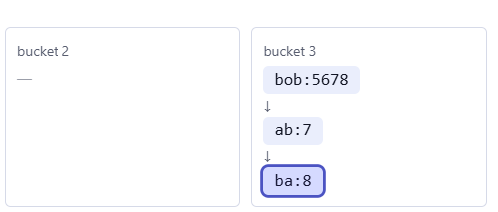
\includegraphics[width=88mm]{fig_web_hash.png}}{Hash map: \mono{bob}, \mono{ab}, \mono{ba} нэг bucket-т унасан collision; хайх алхам бүр харагдана}
\vspace{1.4mm}
\begin{minipage}[t]{0.485\linewidth}
\shot{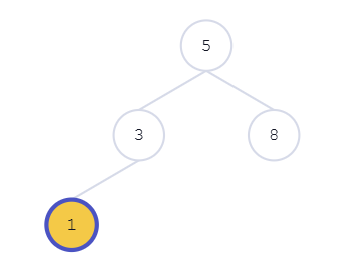
\includegraphics[width=0.84\linewidth]{fig_web_tree.png}}{AVL мод: оруулсан зангилаа тодорч}
\end{minipage}\hfill
\begin{minipage}[t]{0.485\linewidth}
\shot{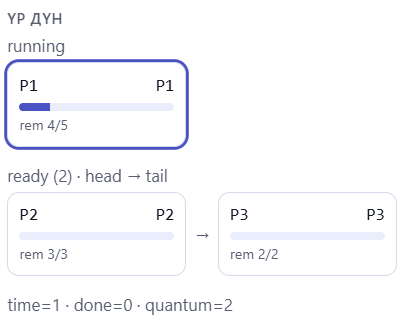
\includegraphics[width=0.84\linewidth]{fig_web_sched.png}}{Round Robin: ready queue тодорч}
\end{minipage}
\end{tcolorbox}
\begin{tcolorbox}[poster={Kernel module -- жинхэнэ Linux дээр}, center lower, height=108mm]
\begin{minipage}[c]{66mm}
\shot{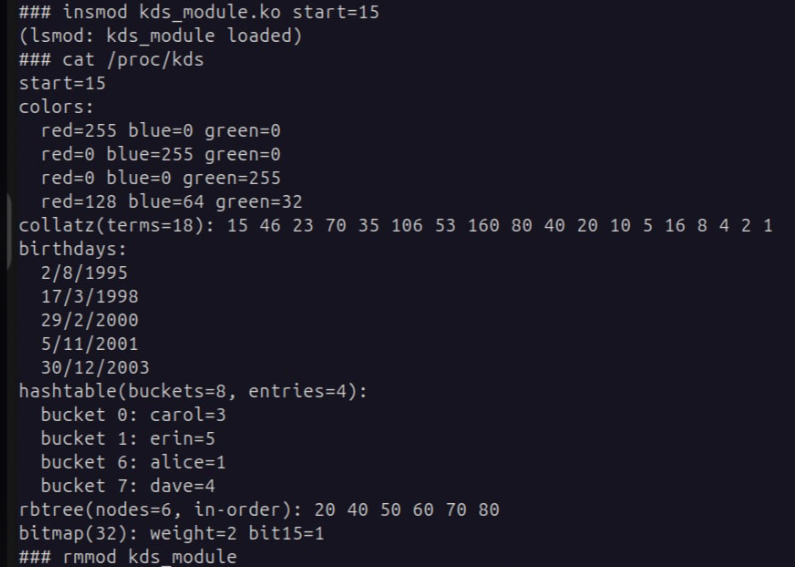
\includegraphics[width=62mm]{fig_kmod15.png}}{\mono{insmod kds\_module.ko start=15}\\ \mono{/proc/kds} ба \mono{dmesg} гаралт}
\end{minipage}\hfill
\begin{minipage}[c]{58mm}
{\small
\begin{itemize}[leftmargin=4mm, itemsep=2.4mm, topsep=0.6mm,
  label={\textcolor{violetA}{\fontsize{7}{7}\selectfont$\blacktriangleright$}}]
\item Ubuntu 24.04.2, \mono{kernel 6.11.0-17-generic}
\item \textbf{Secure Boot} идэвхтэй -- MOK түлхүүрээр гарын үсэг зурсан
\item Part I (color жагсаалт) ба Part II (Collatz: start=25 $\rightarrow$ 24, start=15 $\rightarrow$ 18 гишүүн)
\item \mono{start=0} $\rightarrow$ \mono{-EINVAL}, ачаалагдахгүй
\item \mono{rmmod}: жагсаалт бүрийг \mono{safe} гүйлгээгээр устган
\item Автотест скрипт \textbf{9 PASS}
\end{itemize}\par}
\end{minipage}
\end{tcolorbox}
\begin{tcolorbox}[poster={Scheduler -- Round Robin (q=2)}, center lower, height=108mm]
\centering
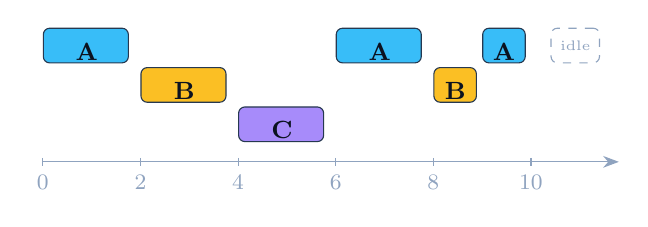
\begin{tikzpicture}[
  x=6.2mm, y=5mm,
  bar/.style={draw=cardline, rounded corners=0.8mm, minimum height=4.4mm,
    anchor=south west},
  lbl/.style={font=\fontsize{7.6}{9}\selectfont, color=muted}
]
\node[bar, minimum width=10.8mm, fill=cyanA]    at (0,2) {};
\node[bar, minimum width=10.8mm, fill=cyanA]    at (6,2) {};
\node[bar, minimum width=5.4mm,  fill=cyanA]    at (9,2) {};
\node[bar, minimum width=10.8mm, fill=amberA]   at (2,1) {};
\node[bar, minimum width=5.4mm,  fill=amberA]   at (8,1) {};
\node[bar, minimum width=10.8mm, fill=violetA]  at (4,0) {};
\node[bar, minimum width=5.4mm, dashed, draw=muted, fill=none] at (10.4,2) {\color{muted}\tiny idle};
\foreach \x/\y/\t in {0.9/2.3/A, 6.9/2.3/A, 9.45/2.3/A, 2.9/1.3/B, 8.45/1.3/B, 4.9/0.3/C}
  \node[font=\fontsize{9}{11}\selectfont, color=bgdark] at (\x,\y) {\bfseries\t};
\draw[-{Stealth[length=2mm]}, color=muted] (0,-0.5) -- (11.8,-0.5);
\foreach \t in {0,2,4,6,8,10} \draw[color=muted] (\t,-0.4) -- (\t,-0.6) node[below, lbl]{\t};
\end{tikzpicture}\\[0.8mm]
{\fontsize{8.8}{11}\selectfont\color{muted}A=5, B=3, C=2 тик, бүгд t=0-д ирсэн -- дуусах 6 / 9 / 10\par}
\vspace{1.2mm}
\begin{tcolorbox}[enhanced, colback=bgdark!85!card, colframe=cardline, arc=1.5mm,
  left=2mm, right=2mm, top=1mm, bottom=1mm]
\centering
{\fontsize{9}{11}\selectfont Дундаж хүлээлт \;\textcolor{amberA}{\bfseries\mono{5.00}} (RR) \;·\; \textcolor{amberA}{\bfseries\mono{4.33}} (FCFS)\par}
\vspace{0.4mm}
{\fontsize{8}{10}\selectfont\color{muted}програм өөрөө \mono{sched stats} командаар тооцдог\par}
\end{tcolorbox}
\end{tcolorbox}

\end{tcbraster}

\vspace{1.5mm}
% ===========================================================================
% МӨР 3: Туршилт · Баг
% ===========================================================================
\begin{tcbraster}[raster columns=3, raster column skip=3.5mm]

\begin{tcolorbox}[poster={Туршилтын хамрах хүрээ}, raster multicolumn=2, height=44mm]
\centering
\stat{98}{make check шалгалт \par бүгд PASS}\hspace{1mm}%
\stat{40\,000}{fuzz команд \par 8 seed × 5000}\hspace{1mm}%
\stat{32}{AVL инвариант \par 30 гүйлт + seed}\hspace{1mm}%
\stat{40}{red-black + heap \par инвариант шалгалт}\hspace{1mm}%
\stat{17}{веб аппын \par Node тест}\hspace{1mm}%
\stat{0}{ASan/UBSan \par алдаа, leak}
\vspace{1mm}
{\centering\begin{minipage}{240mm}\centering
{\fontsize{8.8}{11}\selectfont\color{muted}Stress: 5000 команд × 8 скрипт -- ERR 0, sanitizer мэдээлэлгүй \;·\; CI: GitHub Actions (Ubuntu + macOS) \;·\; 98 PASS шалгалт засварын өмнө ч, дараа ч бүгд PASS -- regression байхгүй\par}
\end{minipage}\par}
\end{tcolorbox}
\begin{tcolorbox}[poster={Гүйцэтгэсэн баг V-1-4}, center lower, height=44mm]
{\small\color{txtw}
\begin{tabular}{@{}p{34mm}@{\hspace{2mm}}p{36mm}@{}}
{\bfseries Н.Ням-Од} {\color{muted}\scriptsize B222270805} &
{\bfseries А.Номин} {\color{muted}\scriptsize B242270088}\\[0.8mm]
{\bfseries А.Гэрэл} {\color{muted}\scriptsize B241940001} &
{\bfseries Э.Мягмаршагай} {\color{muted}\scriptsize B241910001}\\[0.8mm]
{\bfseries О.Хүслэн} {\color{muted}\scriptsize B241910020} &
{\bfseries Ч.Түмэншагай} {\color{muted}\scriptsize B160910830}\\
\end{tabular}\par}
\vspace{1.2mm}
{\small\color{muted}Хичээл заасан багш: {\color{txtw}\bfseries Г.Ганбат} /F.CS10/\par
Улаанбаатар, 2026-11-21\par}
\end{tcolorbox}

\end{tcbraster}

\end{document}
